
\chapter{提案手法}
\label{cpt:提案手法}

\section{概要}

\rad{}が,$l^1$空間で定義したBanach空間上で適用可能である条件は,$DF(\bar{x})$が全単射なことである.

そのために,無限次元ガウスの消去法を用いて,$DF(\bar{x})$が全単射であることを確かめる.

なお,提案手法で用いるBanach空間は,以下のように定義する.

\begin{dfn}[許容重みなしBanach空間$X$]
  \label{dfn:Banach-l1}
  Banach空間$X$を次のように定める.はじめに$l^1$空間を次のように定める.
  \begin{equation}
    l^1 := \left\{ a=(a_k)_{k\in \mathbb{Z}} : a_k \in \mathbb{C}, \|a\| := \sum_{k \in \mathbb{Z}} |a_k| < \infty \right\}
  \end{equation}
  そして,検証に用いる関数空間$X$は
  \begin{equation}
    X:= \mathbb{C} \times l^1, x = (\omega, a), \omega \in \mathbb{C}, a \in l^1
  \end{equation}
  と定め,そのノルムを
  \begin{equation}
    \| x \|_X := \max \{ |\omega| , \|a\| \}
  \end{equation}
  として定義する.このとき,$X$はBanach空間となる.
\end{dfn}

\section{無限次元ガウスの消去法}
$\left \| DF(\bar{x})^{-1} F(\bar{x}) \right \|$について,無限次元ガウスの消去法(節\ref{sct:無限次元ガウスの消去法})を用いる.

\begin{equation*}
  \phi:=DF(\bar{x})^{-1} F(\bar{x})
\end{equation*}
とおくと,
\begin{equation*}
  DF(\bar{x}) \phi = F(\bar{x})
\end{equation*}
と変形できる.$\Pi_N$を射影演算子とすると,
\begin{equation}
    \begin{split}
    \begin{pmatrix}
      \Pi_N DF(\bar{x}) \Pi_N & \Pi_N DF(\bar{x}) (I-\Pi_N) \\
      (I-\Pi_N) DF(\bar{x}) \Pi_N & (I-\Pi_N) DF(\bar{x}) (I-\Pi_N)
    \end{pmatrix}
    \begin{pmatrix}
      \Pi_N \phi \\
      (I-\Pi_N) \phi
    \end{pmatrix}
    \\=
    \begin{pmatrix}
      \Pi_N F(\bar{x}) \\
      (I - \Pi_N) F(\bar{x})
    \end{pmatrix}
  \end{split}
\end{equation}
となり,両辺に$A_M$を掛けて
\begin{equation}
  \label{eq:y0-1}
  \begin{split}
  A_M
    \begin{pmatrix}
      \Pi_N DF(\bar{x}) \Pi_N & \Pi_N DF(\bar{x}) (I-\Pi_N) \\
      (I-\Pi_N) DF(\bar{x}) \Pi_N & (I-\Pi_N) DF(\bar{x}) (I-\Pi_N)
    \end{pmatrix}
    \begin{pmatrix}
      \Pi_N \phi \\
      (I-\Pi_N) \phi
    \end{pmatrix}
    \\=A_M
    \begin{pmatrix}
      \Pi_N F(\bar{x}) \\
      (I - \Pi_N) F(\bar{x})
    \end{pmatrix}
  \end{split}
\end{equation}
となる.

ここで,線形作用素$T,B,C,E$それぞれに対し,
\begin{equation*}
    \label{eq:def_lo}
    \begin{split}
    T:= \Pi_N A_M DF(\bar{x}) \mid _{X_1}:X_1 \rightarrow X_1,\quad &
    B:= \Pi_N A_M DF(\bar{x}) \mid _{X_2}:X_2 \rightarrow X_1, \\
    C:= (I-\Pi_N) A_M DF(\bar{x}) \mid _{X_1}:X_1 \rightarrow X_2,\quad &
    E:= (I-\Pi_N) A_M DF(\bar{x}) \mid _{X_2}:X_2 \rightarrow X_2
  \end{split}
\end{equation*}
と定義でき,式\eqref{eq:y0-1}を次のように変形できる.
\begin{equation}
  \begin{pmatrix}
    T & B \\
    C & E
  \end{pmatrix}
  \begin{pmatrix}
    \Pi_N \phi \\
    (I -\Pi_N) \phi
  \end{pmatrix}
  =
  \begin{pmatrix}
    \Pi_N A_M F(\bar{x}) \\
    (I - \Pi_N) A_M F(\bar{x})
  \end{pmatrix}
\end{equation}

定理\ref{thm:6.2.1-L全単射}より,線形作用素$S$を
\begin{equation*}
  S:=E-CT^{-1}B:X_2 \rightarrow X_2
\end{equation*}
とする.もし,$S$が全単射ならば,
\begin{equation*}
  \begin{pmatrix}
    \Pi_N \phi \\
    (I-\Pi_N)\phi
  \end{pmatrix}
  =
  \begin{pmatrix}
    T^{-1}+T^{-1}BST^{-1} & -T^{-1}BS^{-1} \\
    -S^{-1}CT^{-1} & S^{-1}
  \end{pmatrix}
  \begin{pmatrix}
    Pg \\
    (I-P)g
  \end{pmatrix}
\end{equation*}
となり,有界線形作用素$DF(x)$は全単射となる.

ここで,
\begin{equation}
  \label{eq:I-S_1}
  \| I_{X_2} -S \| < 1
\end{equation}
であれば,$S$は全単射となる.

なお,$DF(x), A_M$の定義は以下の通りである.
\begin{dfn}[拡張したヤコビ行列$DF(x)$]
  \label{dfn:拡張したヤコビ行列}
  まず,近似解$x$について,ある整数$M$を定め,
  \begin{equation}
    x = (\omega,\ \underbrace{0,\cdots,0}_{M},\ a,\ \underbrace{0,\cdots,0}_{M}) \in \mathbb{C}^{2N+2M}
  \end{equation}
  と定めると,$F(x)$のヤコビ行列は
  \begin{equation}
    DF(x) = \left[
      \begin{array}{c|ccc}
        0 & \cdots & 1 & \cdots \\ \hline
        \vdots & & \vdots &  \\
        \partial_w f_k & \cdots & \partial_{a_j}f_k & \cdots \\
        \vdots & & \vdots &
      \end{array}
    \right] %\in \mathbb{C}^{(2N+2M) \times (2N+2M)}
  \end{equation}
  と定義できる.
\end{dfn}
\begin{dfn}[作用素$A_M$の定義]
  \label{dfn:作用素AM}
  はじめに,ある整数$M$を定め,
  \begin{equation}
    \bar{x} = (\omega,\ \underbrace{0,\cdots,0}_{M},\ a,\ \underbrace{0,\cdots,0}_{M}) \in \mathbb{C}^{2N+2M}
  \end{equation}
  と定めると,$A_M$の定義は,以下のように定義できる.
  \begin{equation*}
    A_M = \left(
    \begin{array}{c|ccc}
      DF(\bar{x})^{-1} & 0 & \cdots & \cdots \\ \hline
      0 & \lambda_N^{-1} &  & 0 \\
      \vdots &  & \lambda_{N+1}^{-1} &  \\
      \vdots & 0 &   & \ddots
    \end{array}
    \right)
  \end{equation*}
\end{dfn}


\section{ノルム値の計算}

定義した作用素$T,B,C,E$より,$S$は以下のように変形できる.
\begin{equation}
  \begin{split}
    S =& E-CT^{-1}B \\
    =& \left( \left( I-\Pi_N \right) A_M DF ( \bar{x} ) \right)\\
    &- (\left( I-\Pi_N \right) A_M DF( \bar{x} )) (\Pi_N A_M DF(\bar{x}))^{-1} ((I-\Pi_N)A_M DF(\bar{x}))
  \end{split}
  \label{eq:s-def}
\end{equation}

また,作用素$T,B,C,E$を使って,式\eqref{eq:I-S_1}を変形する.
\begin{equation}
  \label{eq:calc_norm}
  \begin{split}
    \|I_{X_2} - S \| &= \| I_{X_2} - (E-CT^{-1}B)  \| = \| I_{X_2} - E + CT^{-1}B \| \\
    & \leq \| I_{X_2} - E \| + \| C \| \| T^{-1} \| \| B \| \\
    & < 1
  \end{split}
\end{equation}

ここで,各作用素$A_M,DF(\bar{x})$を同じ大きさのブロックに分割する.
\begin{equation}
  A_M = \left[
    \begin{array}{c|ccc}
      DF(\bar{x})^{-1} & 0 & \cdots & \cdots \\ \hline
      0 & \lambda_N^{-1} &  & 0 \\
      \vdots &  & \lambda_{N+1}^{-1} &  \\
      \vdots & 0 &   & \ddots
    \end{array}
    \right]
    = \left[ \begin{array}{c|c}
        T^{-1} & 0 \\ \hline
        0 & \Lambda
    \end{array}\right]
\end{equation}

\begin{equation}
  DF(\bar{x}) = \left[
    \begin{array}{ccc|ccc}
      0 & 1 & \cdots  & 1 & \cdots \\
      \partial_w f_{k} &  \partial_{a_j}f_k & \cdots & \partial_{a_j}f_k & \cdots \\
      \vdots & \vdots & \ddots & \vdots  & \ddots\\ \hline
      \partial_w f_k & \partial_{a_j}f_k & \cdots & \partial_{a_j}f_k & \cdots \\
      \vdots & \vdots & \ddots & \vdots & \ddots
    \end{array}
  \right]
  = \left[ \begin{array}{c|c}
    T & M_{01} \\ \hline
    M_{10} & M_{11}
\end{array} \right]
\end{equation}

このとき,$A_M DF(\bar{x})$はブロック行列を用いて以下のように表せる.なお,ブロック行列のサイズは$\Pi_N$により定まる.

\begin{equation}
  \begin{split}
    A_M DF(\bar{x}) &= \left[ \begin{array}{c|c}
      T^{-1} & 0 \\ \hline
      0 & \Lambda
    \end{array}\right]
    \left[ \begin{array}{c|c}
      T & M_{11} \\ \hline
      M_{21} & M_{22}
    \end{array} \right]
    = \left[ \begin{array}{c|c}
      T^{-1} T & T^{-1}M_{01} \\ \hline
      \Lambda M_{10} & \Lambda M_{11}
    \end{array} \right] \\
    &= \left[ \begin{array}{c|c}
      I & B \\ \hline
      C & E
    \end{array} \right]
  \end{split}
\end{equation}

式\eqref{eq:calc_norm}の各項を,ブロック行列と定義\ref{dfn:拡張したヤコビ行列},\ref{dfn:作用素AM},節\ref{sec:フーリエスペクトル法}を用いて簡単にする.

\begin{enumerate}
  \item[1. $\|I_{X_2} - E \|$]

\begin{equation}
  \tiny
  \begin{split}
    &M_{11}\\
    &=\begin{bmatrix}
      \lambda_{N} & \mu i N \omega (a*a)_{-1} & \cdots & \mu i N \omega (a*a)_{-2N+2} & 0 & \cdots \\
      \mu i (N+1) \omega (a*a)_{1} & \lambda_{N+1} & \cdots & \mu i (N+1) \omega (a*a)_{-2N+1} & \mu i (N+1) \omega (a*a)_{-2N+2} & \cdots \\
      \vdots & \ddots & \ddots & \ddots & \ddots & \ddots \\
      \mu i (3N-2) \omega (a*a)_{2N-2} & \mu i (3N-2) \omega (a*a)_{2N-1} & \ddots & \lambda_{3N-2} & \mu i (3N-2) \omega (a*a)_{-1} & \cdots \\
      0 & \mu i (3N-1) \omega (a*a)_{2N-2} & \ddots & \mu i (3N-1) \omega (a*a)_{1} & \ddots & \ddots \\
      \vdots & \vdots & \vdots & \vdots & \vdots & \ddots \\
    \end{bmatrix}
  \end{split}
\end{equation}
より,

\begin{equation}
  \scriptsize
  \begin{split}
    \|I_{X_2} - E \| =& \| I - \Lambda M_{11}\| \\
    =& \left\| I -
    \begin{bmatrix}
      \lambda^{-1}_N & & \mathbf{0} \\
      & \lambda^{-1}_{N+1} &\\
      \mathbf{0} &  & \ddots
    \end{bmatrix}
    \begin{bmatrix}
      \partial_{a_{N}} f_{N} & \partial_{a_{N+1}} f_{N}  & \cdots \\
      \partial_{a_{N}} f_{N+1} & \partial_{a_{N+1}} f_{N+1}  & \cdots \\
      \vdots & \vdots & \ddots \\
    \end{bmatrix}
    \right\|\\
    =& \left \|
    I - \begin{bmatrix}
      1 & \partial_{a_{N+1}} f_{N}  & \cdots & \lambda^{-1}_{N}\partial_{a_{3N-2}}f_N & 0 & \cdots \\
      \lambda^{-1}_{N+1}\partial_{a_{N}} f_{N+1} & 1  & \ddots & \ddots & \lambda^{-1}_{N+1}\partial_{a_{3N-3}}f_{N+1} & \ddots \\
      \vdots & \ddots & \ddots & \ddots & \ddots & \ddots \\
      \lambda^{-1}_{3N-2}\partial_{a_{N}} f_{3N-2} & \ddots & \ddots & 1 & \ddots & \ddots\\
      0 & \lambda^{-1}_{3N-1}\partial_{a_{N+1}} f_{3N-1}& \ddots & \ddots & 1 & \ddots\\
      \vdots & \ddots & \ddots & \ddots & \ddots & \ddots\\
    \end{bmatrix}
    \right \|\\
    =&\left\|
    \begin{bmatrix}
      0 & \partial_{a_{N+1}} f_{N}  & \cdots & \lambda^{-1}_{N}\partial_{a_{3N-2}}f_N & 0 & \cdots \\
      \lambda^{-1}_{N+1}\partial_{a_{N}} f_{N+1} & 0  & \ddots & \ddots & \lambda^{-1}_{N+1}\partial_{a_{3N-3}}f_{N+1} & \ddots \\
      \vdots & \ddots & \ddots & \ddots & \ddots & \ddots \\
      \lambda^{-1}_{3N-2}\partial_{a_{N}} f_{3N-2} & \ddots & \ddots & 0 & \ddots & \ddots\\
      0 & \lambda^{-1}_{3N-1}\partial_{a_{N+1}} f_{3N-1}& \ddots & \ddots & 0 & \ddots\\
      \vdots & \ddots & \ddots & \ddots & \ddots & \ddots\\
    \end{bmatrix}
    \right \|
  \end{split}
\end{equation}

\begin{equation}
  \begin{split}
    =& \sup \left\{ \right. \\
    &\quad \|\lambda^{-1}_{N+1}\partial_{a_{N}} f_{N+1}\| + \cdots + \|\lambda^{-1}_{3N-2}\partial_{a_{N}} f_{3N-2}\|, \\
    &\quad \|\lambda^{-1}_{N} \partial_{a_{N+1}} f_{N}\| + \cdots + \|\lambda^{-1}_{3N-1}\partial_{a_{N+1}} f_{3N-1}\|,\\
    &\quad \cdots\\
    \left.\right\}\\
    =& \sup \left\{ \right. \\
    &\quad \underbrace{0+ \|\lambda^{-1}_{N+1} \mu i (N+1) \omega (a*a)_{1}\| + \cdots + \|\lambda^{-1}_{3N-2} \mu i (3N-2) \omega (a*a)_{2N-2}\|}_{2N-1}, \\
    &\quad \underbrace{\|\lambda^{-1}_{N}  \mu i N \omega (a*a)_{-1}\| + \cdots + \|\lambda^{-1}_{3N-1} \mu i (3N-1) \omega (a*a)_{2N-2}\|}_{2N},\\
    &\quad \cdots, \\
    &\quad \underbrace{\|\lambda^{-1}_{N}  \mu i N \omega (a*a)_{-2N+2}\| + \cdots + \|\lambda^{-1}_{4N-3} \mu i (4N-3) \omega (a*a)_{2N-2}\|}_{4N-3},\\
    &\quad \underbrace{\|\lambda^{-1}_{N+1}  \mu i (N+1) \omega (a*a)_{-2N+2}\| + \cdots + \|\lambda^{-1}_{4N-2} \mu i (4N-2) \omega (a*a)_{2N-2}\|}_{4N-3},\\
    &\quad \cdots \\
    \left.\right\}
  \end{split}
\end{equation}

上記の上限値は,無限個の要素を比較しなければならない.コンピュータで計算するためには,要素の個数を有限まで小さくする必要がある.そこで,以下の2つの要素
\begin{align}
  &\|\lambda^{-1}_{k}  \mu i k \omega (a*a)_{-2N+2}\| + \cdots + \|\lambda^{-1}_{4k-3} \mu i (4k-3) \omega (a*a)_{2N-2}\|,\\
  &\|\lambda^{-1}_{k+1}  \mu i (k+1) \omega (a*a)_{-2N+2}\| + \cdots + \|\lambda^{-1}_{4k-2} \mu i (4k-2) \omega (a*a)_{2N-2}\|
\end{align}
を比較する.$k\geq N$として,
\begin{equation}
  \begin{split}
    &\|\lambda^{-1}_{k}  \mu i k \omega (a*a)_{-2N+2}\| + \cdots + \|\lambda^{-1}_{4k-3} \mu i (4k-3) \omega (a*a)_{2N-2}\|\\
    &-\|\lambda^{-1}_{k+1}  \mu i (k+1) \omega (a*a)_{-2N+2}\| + \cdots + \|\lambda^{-1}_{4k-2} \mu i (4k-2) \omega (a*a)_{2N-2}\|\\
    =& \left\| \lambda^{-1}_{k}k - \lambda^{-1}_{k+1}(k+1) \right\| \| \mu i \omega (a*a)_{-2N+2}\|+ \cdots \\
    &+ \left\| \lambda^{-1}_{4k-3}(4k-3) - \lambda^{-1}_{4k-2}(4k-2) \right\| \| \mu i \omega (a*a)_{2N-2}\|
  \end{split}
\end{equation}

ここで $ \|\lambda^{-1}_{k}k - \lambda^{-1}_{k+1}(k+1) \|$を計算する.
\begin{equation}
  \begin{split}
    &\|\lambda^{-1}_{k}k - \lambda^{-1}_{k+1}(k+1) \|\\
    =& \left\|\frac{k}{-k^2\omega^2 + \mu i k \omega+ 1} - \frac{k+1}{-(k+1)^2\omega^2 + \mu i (k+1) \omega+ 1}\right\|\\
    =& \left\|\frac{1}{-k\omega^2 + \mu i  \omega+ k^{-1}} - \frac{1}{-(k+1)\omega^2 + \mu i \omega+ (k+1)^{-1}}\right\|\\
    >& 0
  \end{split}
\end{equation}
よって,
\begin{equation}
  \begin{split}
    &\|\lambda^{-1}_{k}  \mu i k \omega (a*a)_{-2N+2}\| + \cdots + \|\lambda^{-1}_{4k-3} \mu i (4k-3) \omega (a*a)_{2N-2}\|\\
    &-\|\lambda^{-1}_{k+1}  \mu i (k+1) \omega (a*a)_{-2N+2}\| + \cdots + \|\lambda^{-1}_{4k-2} \mu i (4k-2) \omega (a*a)_{2N-2}\|\\
    &> 0
  \end{split}
\end{equation}

以上より,要素を省略できて,

\begin{equation}
  \begin{split}
    &\|I_{X_2}-S\|= \sup \left\{ \right. \\
    &\quad \underbrace{0+ \|\lambda^{-1}_{N+1} \mu i (N+1) \omega (a*a)_{1}\| + \cdots + \|\lambda^{-1}_{3N-2} \mu i (3N-2) \omega (a*a)_{2N-2}\|}_{2N-1}, \\
    &\quad \underbrace{\|\lambda^{-1}_{N}  \mu i N \omega (a*a)_{-1}\| + \cdots + \|\lambda^{-1}_{3N-1} \mu i (3N-1) \omega (a*a)_{2N-2}\|}_{2N},\\
    &\quad \cdots, \\
    &\quad \underbrace{\|\lambda^{-1}_{N}  \mu i N \omega (a*a)_{-2N+2}\| + \cdots + \|\lambda^{-1}_{4N-3} \mu i (4N-3) \omega (a*a)_{2N-2}\|}_{4N-3}\\
    &\left.\right\}
  \end{split}
\end{equation}

\item[$\|C\|$]

\begin{equation}
  \tiny
  \begin{split}
    &M_{10}\\
    &= \begin{bmatrix}
      3^{-1}\mu i N (a*a*a)_{N} & 0 & \mu i N \omega (a*a)_{2N-2} & \mu i N \omega (a*a)_{2N-1} & \cdots & \mu i N \omega (a*a)_1 &\\
      3^{-1}\mu i (N+1) (a*a*a)_{N+1} & 0 & 0 & \mu i (N+1) \omega (a*a)_{2N-2} & \cdots & \mu i (N+1) \omega (a*a)_2 &\\
      \vdots & \vdots & \vdots & \ddots & \ddots & \vdots\\
      3^{-1}\mu i (3N-3) (a*a*a)_{3N-3} & 0 & 0 & 0 & \cdots & 0\\
      0 & 0 & 0 & 0 & \cdots & 0 \\
      \vdots & \vdots & \vdots & \vdots & \ddots & \vdots\\
    \end{bmatrix}
  \end{split}
\end{equation}
より,
% lambda M10
\begin{equation}
  \tiny
  \begin{split}
    &\|\Lambda M_{10}\| \\
    &= \left\| \begin{bmatrix}
      \lambda^{-1}_N & & \mathbf{0} \\
      & \lambda^{-1}_{N+1} & \\
      \mathbf{0} &  & \ddots &
    \end{bmatrix}
    \begin{bmatrix}
      \partial_{\omega} f_{N} & \partial_{a_{-N+1}} f_{N} & \cdots \\
      \partial_{\omega} f_{N+1} & \partial_{a_{-N+1}} f_{N+1}  & \cdots \\
      \vdots & \vdots & \ddots \\
    \end{bmatrix} \right\| \\
    &= \left\|  \begin{bmatrix}
      \lambda^{-1}_N & & \mathbf{0} \\
      & \lambda^{-1}_{N+1} & \\
      \mathbf{0} &  & \ddots &
    \end{bmatrix}\right.\\
    & \left.\begin{bmatrix}
      3^{-1}\mu i N (a*a*a)_{N} & 0 & \mu i N \omega (a*a)_{2N-2} & \mu i N \omega (a*a)_{2N-1} & \cdots & \mu i N \omega (a*a)_1 &\\
      3^{-1}\mu i (N+1) (a*a*a)_{N+1} & 0 & 0 & \mu i (N+1) \omega (a*a)_{2N-2} & \cdots & \mu i (N+1) \omega (a*a)_2 &\\
      \vdots & \vdots & \vdots & \ddots & \ddots & \vdots\\
      3^{-1}\mu i (3N-3) (a*a*a)_{3N-3} & 0 & 0 & 0 & \cdots & 0\\
      0 & 0 & 0 & 0 & \cdots & 0 \\
      \vdots & \vdots & \vdots & \vdots & \ddots & \vdots\\
    \end{bmatrix}\right\| \\
  \end{split}
\end{equation}
\begin{equation}
  \begin{split}
    =& \sup \left\{ \right.\\
    &\quad \lambda_N^{-1} 3^{-1}\mu i N (a*a*a)_{N} + 0 + \lambda_{N+2}^{-1} \mu i N \omega (a*a)_{2N-2} + \cdots + \lambda_{N+2}^{-1} \mu i N \omega (a*a)_{},\\
    &\quad \cdots, \\
    &\quad \lambda_{3N-3}^{-1} 3^{-1}\mu i (3N-3) (a*a*a)_{3N-3} \\
    &\left. \right\}
  \end{split}
\end{equation}

\item[$\|T^{-1}\|$]
\begin{equation}
  \begin{split}
    \| T^{-1}\| = \| DF(\bar{x})^{-1}\|
  \end{split}
\end{equation}

\item[$\|B\|$]
% T^{-1}M_{01}q
\begin{equation}
  \begin{split}
    &\|T^{-1}M_{01}\| \\
    =& \left \| \begin{bmatrix}
      T^{-1}_{0\ 0} & \cdots & T^{-1}_{0\ 2N} \\
      \vdots & \ddots & \vdots \\
      T^{-1}_{2N\ 0} & \cdots & T^{-1}_{2N\ 2N} \\
    \end{bmatrix}
    \begin{bmatrix}
      1 & \cdots & \cdots \\
      \partial_{a_N} f_{-N+1} & \partial_{a_{N+1}} f_{-N+1}  & \cdots \\
      \vdots & \vdots & \vdots \\
      \partial_{a_N} f_{N-1} & \partial_{a_{N+1}} f_{N-1}  & \cdots
    \end{bmatrix}\right\| \\
    =& \left\| \begin{bmatrix}
      T^{-1}_{0\ 0} & \cdots & T^{-1}_{0\ 2N} \\
      \vdots & \ddots & \vdots \\
      T^{-1}_{2N\ 0} & \cdots & T^{-1}_{2N\ 2N} \\
    \end{bmatrix}\right.\\
    &\left. \begin{bmatrix}
      1 & \cdots & \cdots  & \cdots & 1 & \cdots \\
      0 & \cdots & \cdots  & \cdots & 0 & \cdots \\
      \mu i (-N+1) \omega (a*a)_{-2N+2} & 0 & \cdots  & \cdots & 0 & \cdots\\
      \mu i (-N+2) \omega (a*a)_{-2N+1} & \mu i (-N+2) \omega (a*a)_{-2N+2} & 0 & \cdots & 0 & \cdots \\
      \vdots & \ddots & \ddots & \ddots & \ddots & \ddots \\
      \mu i (N-1) \omega (a*a)_{-1} & \mu i (N-1) \omega (a*a)_{-2}  & \cdots & \cdots & 0 & \cdots
    \end{bmatrix}\right\|\\
  \end{split}
\end{equation}
\end{enumerate}

上記のノルム値より,$\|I_{X_2} - S\|$をコンピュータで計算する.


\chapter{実験結果}
\section{実験手法}
4章に示した\vdp{}方程式を問題の対象とし,フーリエ・スペクトル法を用いて近似解を計算する.この近似解と\vdp{}方程式を用いて,提案手法で示したノルム値を計算し,$DF(\bar{x})$が全単射であるか確かめる.このとき,フーリエ・スペクトル法におけるフーリエ係数の次数を50,100,150,200と変更し,ノルム値を計算する.

\section{実験環境}
本研究を行った実験環境を表\ref{tab:環境},使用したパッケージを表\ref{tab:パッケージ}を示す.

\begin{table}[h]
  \centering
  \caption{実験環境}
  \label{tab:環境}
  \begin{tabular}{c||c}
    環境 & 詳細 \\ \hline
    CPU & 12th Gen Intel(R) CORE(TM) i7-12700 \\
    OS & Linux(x86_64-linyc-gnu)\\
    Julia & Version 1.11.2
  \end{tabular}
\end{table}

\begin{table}[h]
  \centering
  \caption{使用パッケージ}
  \label{tab:パッケージ}
  \begin{tabular}{c||l}
    パッケージ & バージョン \\  \hline
    DifferentialEquations & v7.10.0 \\
    FFMPEG & v0.4.1 \\
    FFTW & v1.7.1 \\
    ForwardDiff & v0.10.36 \\
    GenericFFT & v0.1.6 \\
    IntervalArithmetic & v0.20.9 \\
    Plots & v1.39.0
  \end{tabular}
\end{table}

\section{実験結果}
実験結果の数値を表\ref{tab:norm-num}に示す.

結果より,フーリエ係数の次数が大きくなるにつれてノルム値が小さくなることがわかる.
また,いかなるフーリエ係数のサイズであっても,ノルム値が$1$を超えることはなかったことがわかる.これは,フーリエ係数のサイズが大きくなるにつれて,計算における$\lambda^{-1}$が小さくなるため,ノルム値が小さくなるためであると考えられる.

この結果より,$DF(\bar{x})$が全単射であることが確かめられた.

\begin{table}[htbp]
  \centering
  \caption{フーリエ係数の次数の変更による$\|I_{X_2}\|$の比較}
  \label{tab:norm-num}
  \begin{tabular}{c||c}
    フーリエサイズ & $\| I_{X_2}-S \|$ \\ \hline
    50 & 0.22815114629236252 \\
    100&0.11455533660051737\\
    150&0.07655718822651922\\
    200&0.05749210273025131
\end{tabular}
\end{table}

\begin{comment}
\begin{figure}[htbp]
  \centering
  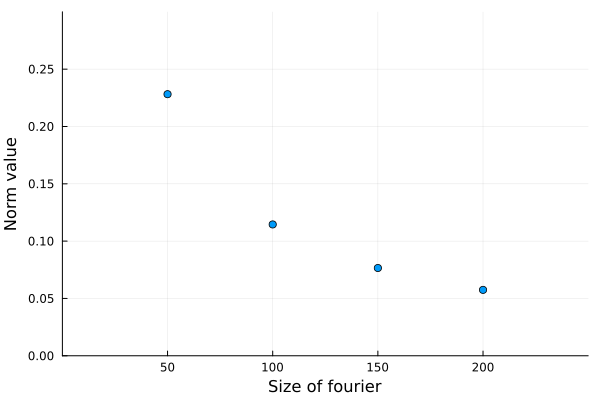
\includegraphics[scale=0.5]{img/scatter.png}
  \caption{フーリエ係数の次数の変更による$\|I_{X_2}\|$の比較}
  \label{fig:norm-gra}
\end{figure}
\end{comment}
